\chapter{Tecniche crittografiche classiche}
\section{Modelli di crittografia simmetica}
La crittografia simmetrica è formata da cinque elementi:
\begin{itemize}
    \item \textbf{Plaintext}: si tratta del testo in chiaro, quindi interpretabile.
    \item \textbf{Algoritmo di cifratura}: l'algoritmo di cifratura esegue 
    varie sostituzioni e trasformazioni del testo in chiaro.
    \item \textbf{Chiave segreta}: la chiave è anch'essa argomento dell'algoritmo 
    di cifratura. La chiave è indipendente dal testo in chiaro e dall'algoritmo. 
    L'algoritmo produrrà un risultato diverso a seconda della specifica chiave utilizzata.
    \item \textbf{Testo cifrato}: Si tratta del messaggio prodotto in output. Dipenderà 
    dal testo in chiaro e dalla chiave segreta. Date due chiavi diverse il risultato 
    in output sarà diverso, genererà quindi due testi cifrati differenti. Il testo 
    cifrato è apparentemente un flusso di dati casuale, sarà quindi illegibile.
    \item \textbf{Algoritmo di decifratura} Si tratta essenzialmente dell'algoritmo 
    di cifratura eseguito inversamente. Prende in input il testo cifrato e la chiave, producendo 
    il testo originale.
\end{itemize}
Ci sono due requisiti per per l'uso sicuro della crittografia convenzionale:
\begin{enumerate}
    \item Abbiamo bisogno di un'algoritmo di cifratura forte. Ciò significa che 
    che chi possiede testi cifrati non sia in grado di trovare facilmente la chiave per
    poterli decifrare.
    \item Il mittente e il destinatario devono aver ricevuto le copie delle chiavi 
    segrete mediante un canale sicuro. Se qualcuno trovasse la chiave conoscendo 
    l'algoritmo, l'intera comunicazione diventerebbe leggibile.
\end{enumerate}
Nella cifratura simmetrica, l'algoritmo di cifratura non deve rimanere segreto, 
ma solo la chiave. Questa caratteristica la rende pratica per un uso diffuso.
I chip di cifratura a basso costo sono ampiamente disponibili e incorporati
in vari prodotti. La principale preoccupazione di sicurezza è mantenere
segreta la chiave.
\subsection{Elementi essenziali di una cifratura simmetrica}
\begin{itemize}
    \item Una sorgente produce un messaggio in testo in chiaro $X = [X_1, X_2, \ldots, X_M]$.
    \item Viene generata una chiave di cifratura $K = [K_1, K_2, \ldots, K_J]$, che deve essere mantenuta segreta.
    \item Con il messaggio $X$ e la chiave $K$ come input, l'algoritmo di cifratura genera 
    il testo cifrato $Y = [Y_1, Y_2, \ldots, Y_N]$, rappresentato come $Y = E(K, X)$.
    \item Il destinatario inteso, in possesso della chiave, può decifrare il messaggio: $X = D(K, Y)$.
\end{itemize}

\subsection{Sicurezza}
Un avversario che osserva $Y$ senza conoscere $K$ o $X$ può tentare di recuperare $X$ o $K$. 
È presumibile che l'avversario conosca gli algoritmi di cifratura (E) e decifratura (D).
Se l'avversario è interessato solo a un messaggio specifico, si concentrerà sul recupero
di $X$. Tuttavia, se desidera leggere futuri messaggi, cercherà di recuperare $K$.

\subsection{Crittografia}
I sistemi crittografici possono essere caratterizzati lungo tre dimensioni
indipendenti:
\begin{enumerate}
    \item \textbf{Il tipo di operazioni utilizzate per trasformare il testo in chiaro
    in testo cifrato}. Tutti gli algoritmi di cifratura si basano su due principi
    generali: la sostituzione, in cui ciascun elemento nel testo in 
    chiaro (\textit{bit, lettera, gruppo di bit o lettere}) è mappato
    in un altro elemento, e la trasposizione, in cui gli elementi nel
    testo in chiaro vengono riarrangiati. Il requisito fondamentale è
    che non venga persa alcuna informazione (\textit{ossia, che tutte
    le operazioni siano reversibili}). La maggior parte dei sistemi,
    chiamati sistemi a prodotto, coinvolge multiple fasi di sostituzioni
    e trasposizioni.
    \item \textbf{Il numero di chiavi utilizzate}. Se mittente e destinatario
    utilizzano la stessa chiave, il sistema è chiamato simmetrico,
    a chiave singola, a chiave segreta o cifratura convenzionale.
    Se mittente e destinatario utilizzano chiavi diverse, il sistema
    è chiamato asimmetrico, a due chiavi o cifratura a chiave pubblica.
    \item \textbf{Il modo in cui il testo in chiaro viene processato}. Una cifra
    a blocchi processa l'input un blocco di elementi alla volta, producendo
    un blocco di output per ciascun blocco in input. Una cifra a flusso
    processa gli elementi in input in modo continuo, producendo l'output
    elemento per elemento man mano che procede.
\end{enumerate}

Solitamente, l'obiettivo nell'attaccare un sistema di crittografia è di recuperare la chiave
in uso anziché semplicemente ottenere il testo in chiaro di un singolo testo cifrato. Esistono
due approcci generali per attaccare uno schema di crittografia convenzionale:

\begin{enumerate}
    \item \textbf{Criptoanalisi:} Gli attacchi crittoanalitici si basano sulla natura
    dell'algoritmo e talvolta su qualche conoscenza delle caratteristiche generali del
    testo in chiaro o anche su alcune coppie di testo in chiaro - testo cifrato di esempio.
    Questo tipo di attacco sfrutta le caratteristiche dell'algoritmo per cercare
    di dedurre un testo in chiaro specifico o la chiave in uso.
    \item \textbf{Attacco a Forza Bruta:} L'attaccante prova ogni possibile chiave su
    un testo cifrato finché non ottiene una traduzione intelligibile in testo in chiaro. In media,
    è necessario provare la metà di tutte le chiavi possibili per avere successo.
\end{enumerate}

Se uno dei due tipi di attacco riesce a dedurre la chiave, l'effetto è catastrofico:
tutti i messaggi futuri e passati crittografati con quella chiave sono compromessi.

Il primo tipo di attacco, la criptoanalisi, si basa sulla conoscenza dell'algoritmo
e delle caratteristiche del testo in chiaro o su coppie di testo in chiaro - testo cifrato di esempio.
L'obiettivo è dedurre il testo in chiaro o la chiave in uso. L'altro tipo di attacco è basato
sulla forza bruta, dove vengono provate tutte le possibili chiavi fino a trovare
una traduzione intelligibile del testo cifrato.

L'attacco basato solo sul testo cifrato è il più facile da difendere perché l'avversario
ha la minore quantità di informazioni con cui lavorare. Tuttavia, in molti casi,
l'analista dispone di più informazioni. L'analista potrebbe essere in grado di catturare
uno o più messaggi in testo in chiaro insieme alle loro cifrature. Oppure l'analista potrebbe
sapere che certi modelli di testo in chiaro appariranno in un messaggio. Ad esempio,
un file codificato in formato PostScript inizia sempre con lo stesso modello,
o potrebbe esserci un'intestazione o un banner standardizzato in un messaggio
di trasferimento di fondi e così via. Tutti questi sono esempi di testo in chiaro
conosciuti. Con questa conoscenza, l'analista potrebbe essere in grado di dedurre
la chiave in base al modo in cui il testo in chiaro noto viene trasformato.

Strettamente correlato all'attacco basato sul testo in chiaro conosciuto è quello
che potrebbe essere definito come un attacco basato su parole probabili.
Se l'avversario sta lavorando con la crittografia di un messaggio di prosa
generale, potrebbe avere poca conoscenza di ciò che è nel messaggio. Tuttavia,
se l'avversario sta cercando informazioni molto specifiche, potrebbero essere
noti alcuni pezzi del messaggio. Ad esempio, se viene trasmesso un intero
file contabile, l'avversario potrebbe conoscere la posizione di alcune parole
chiave nell'intestazione del file. Come altro esempio, il codice sorgente
di un programma sviluppato dalla Corporation X potrebbe includere una
dichiarazione di copyright in una posizione standardizzata. Se l'analista
è in grado in qualche modo di far inserire al sistema sorgente un messaggio
scelto dall'analista, allora è possibile un attacco basato sul testo in chiaro
scelto. Un esempio di questa strategia è la crittoanalisi differenziale.
In generale, se l'analista è in grado di scegliere i messaggi da cifrare,
potrebbe deliberatamente selezionare modelli che possono essere previsti
per rivelare la struttura della chiave.

Due altri tipi di attacco elencati sono testo cifrato scelto e testo scelto,
che sono meno comuni ma possibili. Solo algoritmi relativamente deboli non
resistono a un attacco basato solo sul testo cifrato. In generale, un algoritmo
di crittografia è progettato per resistere a un attacco basato sul testo in chiaro
conosciuto. Uno schema di crittografia è incondizionatamente sicuro se il
testo cifrato generato dallo schema non contiene informazioni sufficienti
per determinare univocamente il testo in chiaro corrispondente, indipendentemente
dalla quantità di testo cifrato disponibile. Cioè, non importa quanto tempo abbia
un avversario, è impossibile per lui o lei decifrare il testo cifrato
semplicemente perché le informazioni necessarie non ci sono. Con
l'eccezione di uno schema noto come ``one-time pad", non esiste
un algoritmo di crittografia che sia incondizionatamente sicuro.
Pertanto, tutto ciò a cui gli utenti di un algoritmo di crittografia
possono aspirare è un algoritmo che soddisfi una o entrambe delle
seguenti criteri:

\begin{enumerate}
    \item Il costo per rompere la cifra supera il valore delle informazioni
    crittografate.
    \item Il tempo richiesto per rompere la cifra supera la vita utile
    delle informazioni.
\end{enumerate}

Uno schema di crittografia è considerato sicuro computazionalmente se
soddisfa una qualsiasi delle due precedenti criteri. Sfortunatamente,
è molto difficile stimare la quantità di sforzo necessaria per
crittoanalizzare con successo il testo cifrato.

Tutte le forme di crittoanalisi per gli schemi di crittografia
simmetrica sono progettate per sfruttare il fatto che tracce di
struttura o modello nel testo in chiaro possono sopravvivere alla crittografia
e possono essere discernibili nel testo cifrato.
\section{Tecniche di sostituzione}
I due elementi base di tutte le tecniche di crittografia sono la sostituzione e 
la trasposizione.

Una tecnica di sostituzione è una tecnica in cui le lettere del testo in chiaro vengono 
sostituite da altre lettere o da numeri o simboli. Se il testo in chiaro 
viene visto come una sequenza di bit, allora la sostituzione comporta la sostituzione 
di modelli di bit del testo in chiaro con modelli di bit di testo cifrato.
\subsection{Cifrario di cesare}
Il cifrario di Cesare è noto come il primo e più semplice esempio di
cifrario a sostituzione. Fu utilizzato da Giulio Cesare e coinvolge la
sostituzione di ogni lettera dell'alfabeto con la lettera situata tre
posizioni più in basso nell'alfabeto. Ad esempio:

\begin{center}
\begin{tabular}{|c|c|}
\hline
\textbf{Plain} & \textbf{Ciphertext} \\
\hline
a & D \\
b & E \\
c & F \\
d & G \\
e & H \\
f & I \\
g & J \\
h & K \\
i & L \\
j & M \\
k & N \\
l & O \\
m & P \\
\hline
\end{tabular}
\hspace{2cm}
\begin{tabular}{|c|c|}
\hline
\textbf{Plain} & \textbf{Ciphertext} \\
\hline
n & Q \\
o & R \\
p & S \\
q & T \\
r & U \\
s & V \\
t & W \\
u & X \\
v & Y \\
w & Z \\
x & A \\
y & B \\
z & C \\
\hline
\end{tabular}
\end{center}

È importante notare che l'alfabeto è avvolto in modo che la lettera
successiva a Z sia A. Ogni lettera dell'alfabeto viene quindi sostituita
dalla lettera che si trova a tre posizioni più in basso.

Il cifrario di Cesare è un esempio semplice ma storico di crittografia a
sostituzione. Può essere utilizzato per crittografare un messaggio
spostando ogni lettera di tre posizioni nell'alfabeto.

L'algoritmo utilizzato è il seguente:
\[
C = E(3, p) = (p + 3)\mod 26  
\]
Lo shift potrebbe essere un valore generico $k$, quindi l'agoritmo generalizzato 
è:
\[
C = D(k, p) = (p + k)\mod 26  
\]
ove $k$ prende un valore nel compreso tra $1$ e $25$. L'algoritmo di 
decifrazione è simile:
\[
  p = D(k, C) = (C - k)\mod 26  
\]

Se è noto che un certo testo cifrato è un cifrario di Cesare, allora 
una crittoanalisi a forza bruta è facilmente eseguibile: basta provare
tutte e 25 le possibili chiavi. La Figura 2.3 mostra i risultati di
questa strategia applicata all'esempio di ciphertext. In questo caso,
il plaintext salta fuori occupando la terza linea.

Tre importanti caratteristiche di questo problema ci hanno permesso
di utilizzare una crittoanalisi a forza bruta:
\begin{enumerate}
    \item Gli algoritmi di cifratura e decifratura sono noti.
    \item Ci sono solo $25$ chiavi da provare.
    \item La lingua del plaintext è nota ed è facilmente riconoscibile.
\end{enumerate}

La crittoanalisi a forza bruta è un metodo efficace quando si tratta
di cifrari di Cesare, in quanto le limitate possibilità di chiavi e
la conoscenza dell'algoritmo semplificano notevolmente il processo
di decrittografia.

Nella maggior parte delle situazioni di networking, possiamo presumere
che gli algoritmi siano noti. Quello che rende generalmente impraticabile
la crittoanalisi a forza bruta è l'uso di un algoritmo che impiega un
grande numero di chiavi. Ad esempio, l'algoritmo Triple DES, esaminato
nel Capitolo 6, utilizza una chiave di 168 bit, che crea uno spazio
delle chiavi di $2^{168}$ o più di $3.7 \times 10^{50}$ possibili
chiavi.

La terza caratteristica è anche significativa. Se la lingua del
plaintext è sconosciuta, allora l'output del plaintext potrebbe non
essere riconoscibile. Inoltre, l'input potrebbe essere abbreviato o
compresso in qualche modo, rendendo di nuovo difficile il riconoscimento.
\subsection{Cifrario  monoalfabetico}
Con solo 25 chiavi possibili, il cifrario di Cesare è molto lontano
dall'essere sicuro. Un aumento drammatico dello spazio delle chiavi
può essere ottenuto consentendo una sostituzione arbitraria. Prima
di procedere, definiamo il termine ``permutazione".
\begin{tcolorbox}[title = {Permutazione}]
Una permutazione di un insieme finito di elementi $S$ è una
sequenza ordinata di tutti gli elementi di $S$, con ciascun elemento
che appare esattamente una volta. Ad esempio, se $S = \{a, b, c\}$, ci
sono sei permutazioni di $S$:
\end{tcolorbox}
\[
abc, acb, bac, bca, cab, cba
\]
In generale, ci sono $n!$ permutazioni di un insieme
di $n$ elementi, poiché il primo elemento può essere scelto in uno
dei modi $n$ possibili, il secondo in $n - 1$ modi, il terzo
in $n - 2$ modi e così via.

Ricordiamo l'assegnazione per il cifrario di Cesare:
\begin{center}
\begin{tabular}{|c|c|}
\hline
\textbf{Plain} & \textbf{Ciphertext} \\
\hline
a & D \\
b & E \\
c & F \\
d & G \\
e & H \\
f & I \\
g & J \\
h & K \\
i & L \\
j & M \\
k & N \\
l & O \\
m & P \\
\hline
\end{tabular}
\end{center}

Se invece la linea ``ciphertext" può essere qualsiasi permutazione
dei $26$ caratteri alfabetici, allora ci sono $26!$ o più di $4 \times 10^{26}$
possibili chiavi. Questo è $10$ ordini di grandezza superiore all
spazio delle chiavi per \verb|DES| e sembrerebbe eliminare le tecniche di
crittoanalisi a forza bruta. Un approccio del genere è chiamato
cifrario di sostituzione monoalfabetica, perché viene utilizzato
un singolo alfabeto cifrato (\textit{mappatura dall'alfabeto in chiaro
all'alfabeto cifrato}) per ogni messaggio.

C'è, tuttavia, un'altra linea di attacco. Se il crittoanalista
conosce la natura del testo in chiaro (\textit{ad esempio, testo inglese
non compresso}), può sfruttare le regolarità della lingua. Per vedere
come potrebbe procedere tale crittoanalisi, diamo qui un esempio
parziale adattato da uno in \verb|[SINK09]|. Il testo cifrato da
risolvere
è il seguente:
\begin{verbatim}
UzqSovUoHxmoPvgPozPevSgzWSzoPfPeSxUDBmeTSxaIz
vUePHzHmDzSHzoWSfPaPPDTSvPqUzWymxUzUHSx
ePyePoPDzSzUfPomBzWPfUPzHmDJUDTmoHmq
\end{verbatim}
Come primo passo, può essere determinata la frequenza relativa delle
lettere e confrontata con una distribuzione di frequenza standard per
l'inglese.
Se il messaggio fosse abbastanza lungo, questa tecnica da sola potrebbe
essere sufficiente, ma poiché questo è un messaggio relativamente breve,
non possiamo aspettarci una corrispondenza esatta. In ogni caso, le
frequenze relative delle lettere nel testo cifrato (\textit{in percentuale}) sono
le seguenti:
\begin{figure}[H]
    \centering
    \begin{tabular}{cccc}
        P 13.33 & Z 11.67 & S 8.33 & U 8.33 \\
        O 7.50 & M 6.67 & H 5.83 & D 5.00 \\
        E 5.00 & V 4.17 & X 4.17 & F 3.33 \\
        W 3.33 & Q 2.50 & T 2.50 & A 1.67 \\
        B 1.67 & G 1.67 & Y 1.67 & I 0.83 \\
        J 0.83 & C 0.00 & K 0.00 & L 0.00 \\
        N 0.00 & R 0.00 &
    \end{tabular}
\end{figure}

\begin{figure}[H]
    \centering
    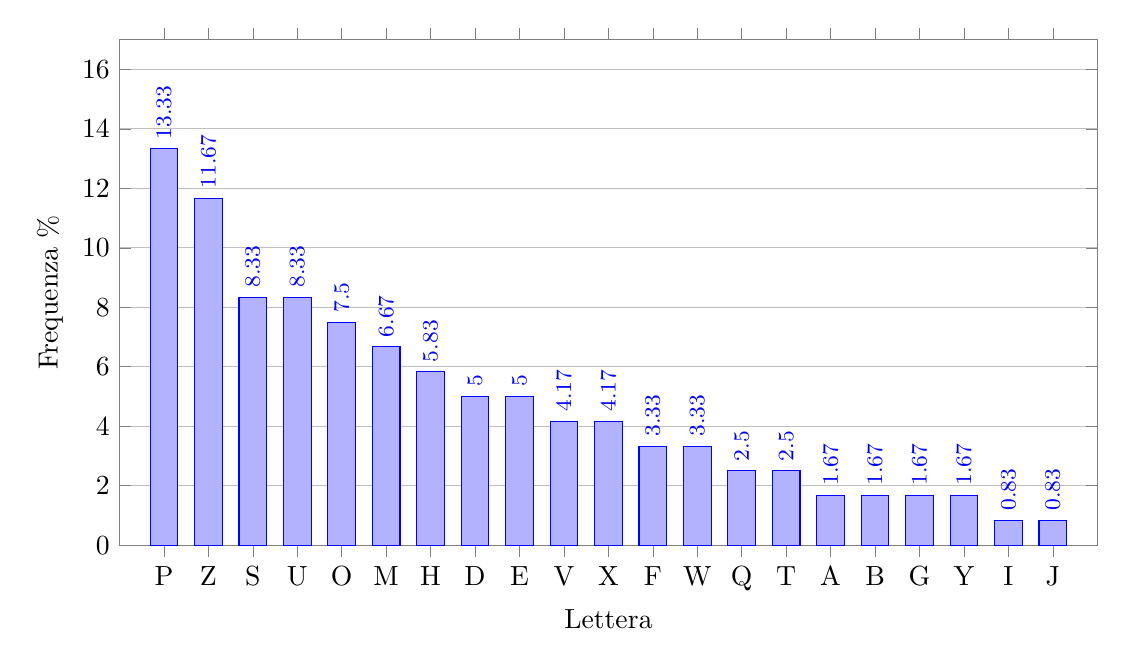
\begin{tikzpicture}
        \begin{axis}[
            ybar,
            ylabel=Frequenza \%,
            xlabel=Lettera,
            symbolic x coords={P, Z, S, U, O, M, H, D, E, V, X, F, W, Q, T, A, B, G, Y, I, J},
            xtick=data,
            nodes near coords,
            nodes near coords align={vertical}, % Imposta l'allineamento verticale dei numeri delle coordinate
            nodes near coords style={rotate=90}, % Ruota i numeri delle coordinate in verticale
            nodes near coords style={right, font=\footnotesize}, % Posiziona i numeri sopra le barre e riduce la dimensione del carattere
            width=14cm,
            height=8cm,
            enlarge x limits=0.05,
            ymin=0,
            ymax=17,
            ymajorgrids=true,
            bar width=10pt, % Larghezza delle barre
            axis line style={gray}, % Imposta il colore dell'asse su grigio
            y axis line style={gray}, % Imposta il colore dell'asse y su grigio
        ]
        \addplot coordinates {
            (P,13.33)
            (Z,11.67)
            (S,8.33)
            (U,8.33)
            (O,7.50)
            (M,6.67)
            (H,5.83)
            (D,5.00)
            (E,5.00)
            (V,4.17)
            (X,4.17)
            (F,3.33)
            (W,3.33)
            (Q,2.50)
            (T,2.50)
            (A,1.67)
            (B,1.67)
            (G,1.67)
            (Y,1.67)
            (I,0.83)
            (J,0.83)
        };
        \end{axis}
        \end{tikzpicture}
        \caption{Frequenze relative alle lettere nei testi inglesi}
\end{figure}
